\newpage
\maketitle
\begin{center}
\Large \textbf{第1章 行情数据处理} \quad 
\end{center}
\begin{abstract}
在本章中我们将通过AKshare库,获取A股分钟级行情数据,并将其进行预处理,变为深度学习可用的数据集。
\end{abstract}
\section{行情数据处理概述}
\subsection{获取原始行情数据}
我们首先通过apps.fmts.ds.akshare\_data\_source.AkshareDataSource获取原始的行情数据,-将其保存到csv文件中。如果存在该csv文件,则
直接从该文件中读出数据并返回。数据格式为:
\lstset{language=PYTHON, caption={行情数据格式}, label={c001-quotation-1-minute-bar}, basicstyle = \ttfamily}
\begin{lstlisting}
......
['2021-08-17 14:55:00', 30.339999999999996, 30.339999999999996, 30.339999999999996, 30.339999999999996, 200.0]
['2021-08-17 14:55:01', 30.339999999999996, 30.339999999999996, 30.339999999999996, 30.339999999999996, 200.0]
......
\end{lstlisting}
\subsection{行情数据预处理}
\subsubsection{价格折线图}
我们以收盘价为例,收盘价的折线图绘制程序如下所示:
\lstset{language=PYTHON, caption={收盘价折线图}, label={c001-close-price-curve-001}, basicstyle = \ttfamily}
\begin{lstlisting}
    class OhlcvProcessor(object):
    # 价格折线图模式
    PCM_DATETIME = 1
    PCM_TICK = 2

    @staticmethod
    def draw_close_price_curve(stock_symbol: str, mode=1) -> None:
        '''
        绘制收盘价折线图,横轴为时间,纵轴为收盘价
        '''
        data = AkshareDataSource.get_minute_bars(stock_symbol=stock_symbol)
        x = [v[0] for v in data[0:1000]]
        y = [v[4] for v in data[0:1000]]
        if mode == OhlcvProcessor.PCM_DATETIME:
            OhlcvProcessor._draw_date_price_curve(x, y)
        else:
            OhlcvProcessor._draw_tick_price_curve(y)

    def _draw_date_price_curve(x: List, y: List) -> None:
        x = [datetime.datetime.strptime(di, '%Y-%m-%d %H:%M:%S') for di in x]
        fig, axes = plt.subplots(1, 1, figsize=(8, 4))
        plt.rcParams['font.sans-serif']=['SimHei'] #用来正常显示中文标签
        plt.rcParams['axes.unicode_minus'] = False #用来正常显示负号
        # 最大化绘图窗口
        figmanager = plt.get_current_fig_manager()
        figmanager.window.state('zoomed')    #最大化
        # 绘制收盘价格折线图
        axes.plot_date(x, np.array(y), '-', label='Net Worth')
        # 设置横轴时间显示格式
        axes.xaxis.set_major_formatter(DateFormatter('%Y-%m-%d %H:%M:%S'))
        plt.gcf().autofmt_xdate()
        # 显示图像
        plt.show()
    
    def _draw_tick_price_curve(y: List) -> None:
        x = range(len(y))
        fig, axes = plt.subplots(1, 1, figsize=(8, 4))
        plt.rcParams['font.sans-serif']=['SimHei'] #用来正常显示中文标签
        plt.rcParams['axes.unicode_minus'] = False #用来正常显示负号
        # 最大化绘图窗口
        figmanager = plt.get_current_fig_manager()
        figmanager.window.state('zoomed')    #最大化
        # 绘制收盘价格折线图
        plt.title('收盘价折线图')
        axes.set_xlabel('时间刻度')
        axes.set_ylabel('收盘价')
        axes.plot(x, np.array(y), '-', label='Net Worth')
        plt.show()
\end{lstlisting}
代码解读如下所示:
\begin{itemize}
    \item 第3、4行:定义收盘价曲线绘制方式,一种是横轴为时间,另一种横轴为行情序号;
    \item 第6$\sim$10行:定义收盘价绘制方法,参数为股票代码和绘制模式,缺省值为横轴为时间(以分钟为单位),这种模式的缺点是从上一日收盘到下一日开盘有
    较大的时间间隔;
    \item 第11行:获取分钟线行情数据,格式为:[[dateteime, open, high, low, close, volume]];
    \item 第19行:以横轴为行情时间值绘制收盘价曲线;
    \begin{itemize}
        \item 第20行:将时间变为'2021-08-21 12:56:00'格式的列表;
        \item 第21行:设置显示图形;
        \item 第22行:设置字体使matplotlib可以正确显示汉字;
        \item 第23行:使matplotlib可以显示负号;
        \item 第24$\sim$26行:使matplotlib绘图窗口最大化;
        \item 第27、28行:绘制收盘价时间曲线;
        \item 第29$\sim$31行:设置横坐标轴时间显示格式为'2021-08-21 12:56:00',并自动调整为45度角倾斜,以节省显示空间;
    \end{itemize}
\end{itemize}
\begin{figure}[H]
	\caption{以时间为横轴的收盘价折线图}
	\label{f000001}
	\centering
	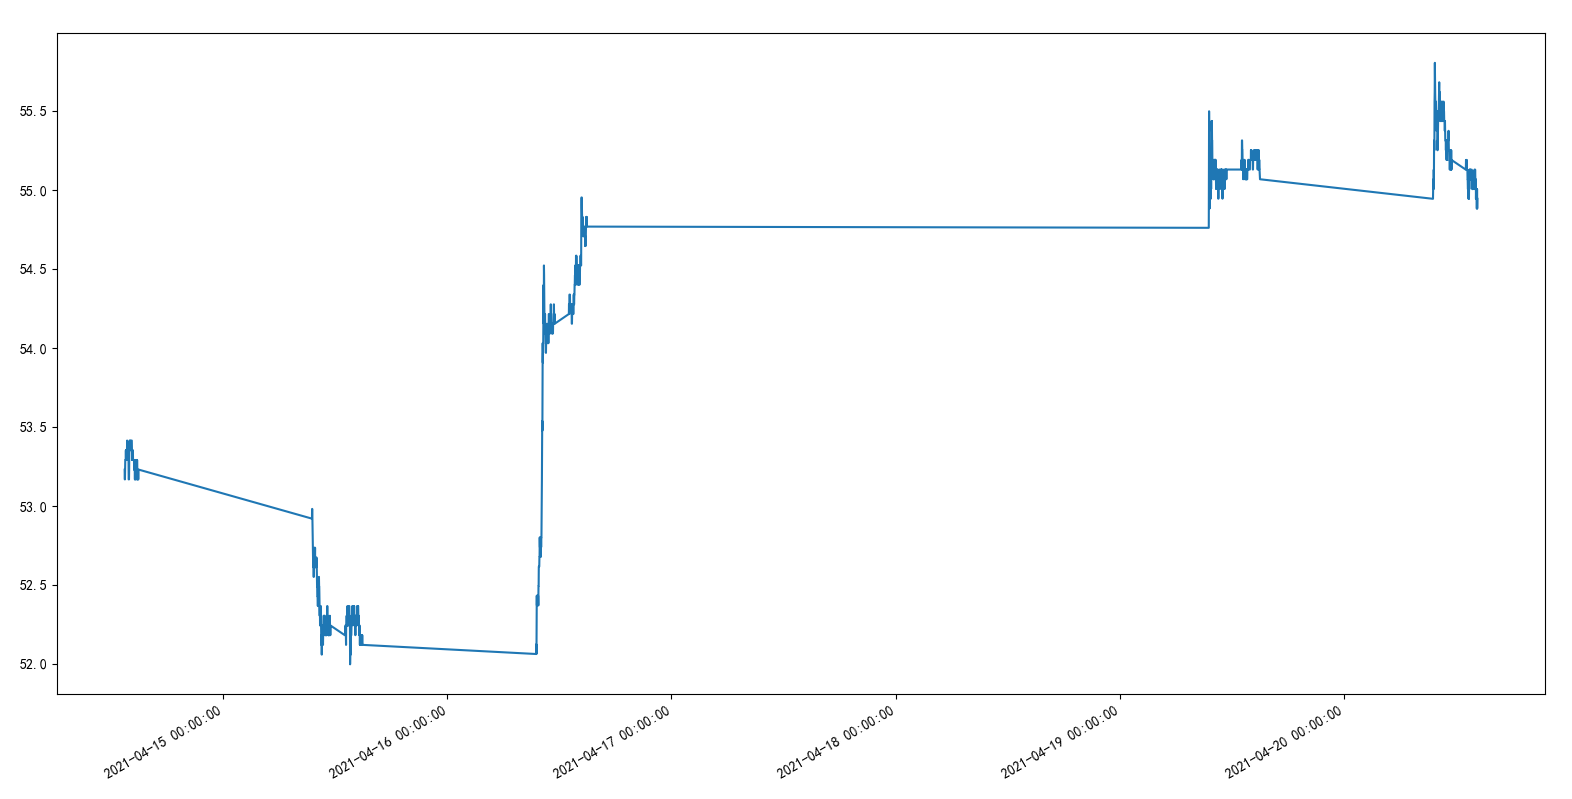
\includegraphics[width=10cm]{images/f000001}
\end{figure}
\begin{figure}[H]
	\caption{以序号为横轴的收盘价折线图}
	\label{f000002}
	\centering
	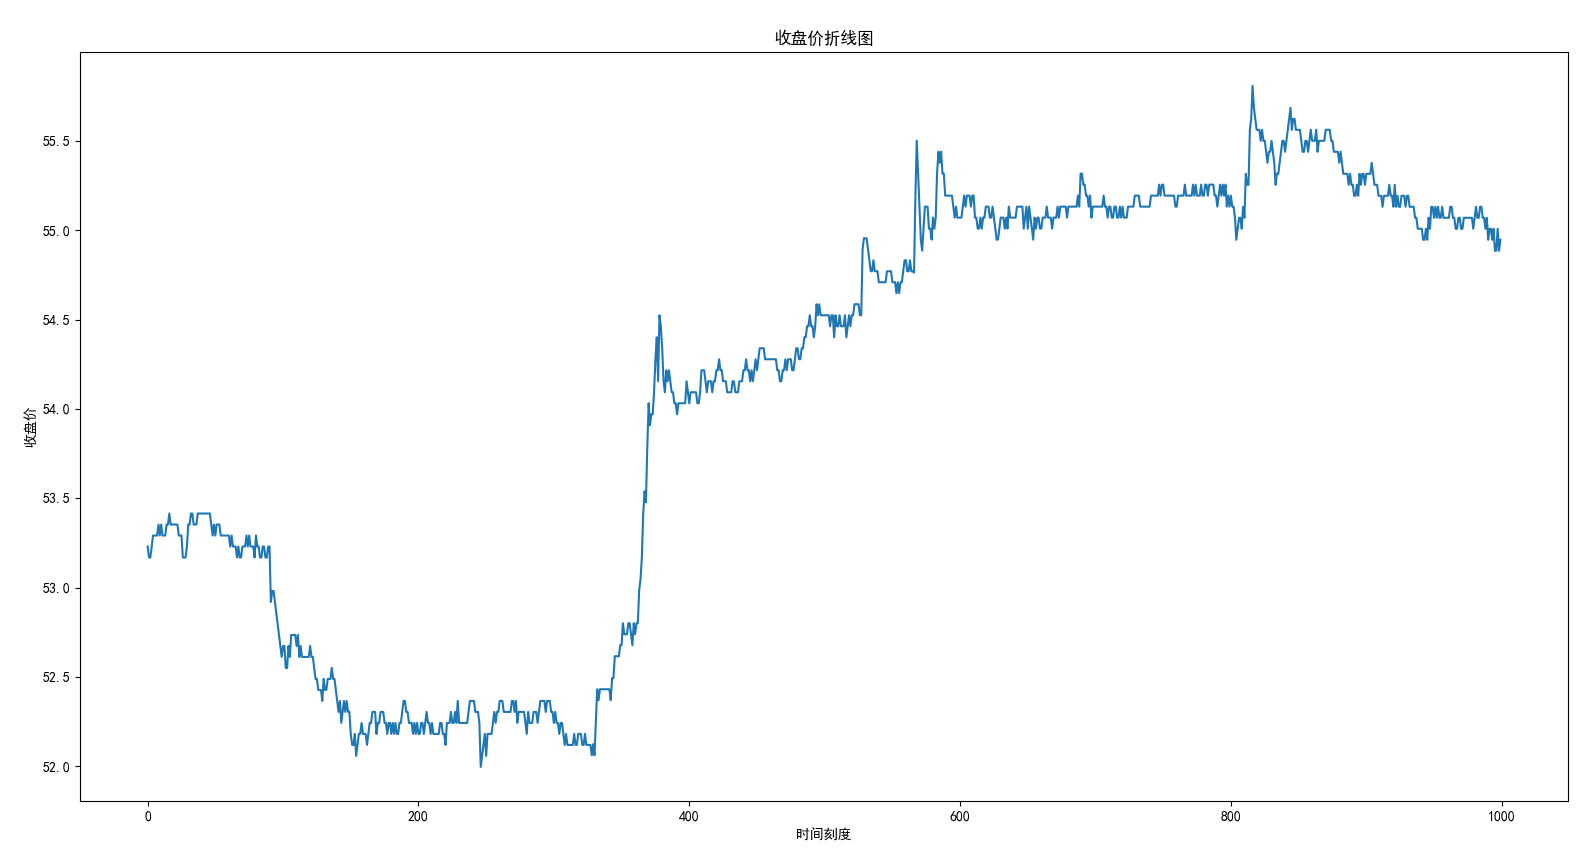
\includegraphics[width=10cm]{images/f000002}
\end{figure}
如\ref{f000001}所示,图中每天收盘到第二天开盘间没有行情数据,所以图形不太好看出规律,而图\ref{f000002}则可以较好的反映价格的变化规律,因此
我们在通常情况下,选择图\ref{f000002}的形式。
\subsubsection{对数差分序列}
我们都知道,原始的行情数据,不具备平稳性,即无法通过历史数据来预测未来,而对数差分序列则具有平稳性,可以用来进行预测。如下所示:
\lstset{language=PYTHON, caption={收盘价折线图}, label={c001-close-price-curve-001}, basicstyle = \ttfamily}
\begin{lstlisting}
    @staticmethod
    def gen_1d_log_diff_norm(stock_symbol, items):
        '''
        从原始行情数据,求出一阶对数收益率log(day2)-log(day1),然后求出每列均值和标准差,利用
        (x-mu)/std进行标准化,分别保存原始信息和归整后信息
        参数:
            stock_symbol 股票编号
            items 由AkshareDataSource.get_minute_bars方法获取到
        '''
        datas = np.array([x[1:] for x in items])
        log_ds = np.log(datas)
        log_diff = np.diff(log_ds, n=1, axis=0)
        log_diff_mu = np.mean(log_diff, axis=0)
        log_diff_std = np.std(log_diff, axis=0)
        ld_ds = (log_diff - log_diff_mu) / log_diff_std
        # 保存原始信息
        raw_file = './apps/fmts/data/{0}_1m_raw.txt'.format(stock_symbol)
        with open(raw_file, 'w', encoding='utf-8') as fd:
            for item in items[1:]:
                fd.write('{0},{1},{2},{3},{4},{5}\n'.format(item[0], item[1], 
                            item[2], item[3], item[4], item[5]))
        # 保存规整化后数据
        ld_file = './apps/fmts/data/{0}_1m_ld.csv'.format(stock_symbol)
        np.savetxt(ld_file, ld_ds)

# 测试程序
    def test_gen_1d_log_diff_norm_001(self):
        stock_symbol = 'sh600260'
        items = AkshareDataSource.get_minute_bars(stock_symbol=stock_symbol)
        OhlcvProcessor.gen_1d_log_diff_norm(stock_symbol, items)
\end{lstlisting}
代码解读如下所示:
\begin{itemize}
    \item 第2行:items由AkshareDataSource.get\_minute\_bars方法获取到,格式为[..., ['2021-08-19 15:00:00', 1.1, 1.5, 1.0, 1.2, 1000], ...];
    \item 第10行:把items中的条目,去除掉日期列后,生成ndarray;
    \item 第11行:对所有元素取对数,以自然数e为底,np.log2是以2底,np.log10是以10为底;
    \item 第12行:取一阶差分,其中n=1代表是一阶差分,即后面一个元素减前面一个元素,out[i] = x[i+1]-x[i],因为axis=0,所以i代表行;
    \item 第13行:求出行方向的均值;
    \item 第14行:求出行方向的标准差;
    \item 第15行:进行归一化:$\hat{x}=\frac{x-\mu}{\sigma}$;
    \item 第18~21行:保存原始的行情信息,因为取了一阶差分,所以去掉了第1行;
    \item 第23、24行:保存一阶差分规整化后的数据;
\end{itemize}
\subsection{数据集支撑数据}
在每一个时间点,我们向前看window\_size个时间点,缺省是10个,然后再加上当前时间点的数据:开盘、最高、最低、收盘、交易量,所以共有$10 \times 5 + 5 = 55$个数据,
我们的算法会根据这55维向量,我们以当前时刻收盘价为标准,确定判断为上涨趋势的最低价格(一旦超过该值即视为上涨),判断为下跌的最高价格(一旦低于该值即视为下跌),向后
连续读取指定个时刻,缺省值为100,如果未来价格首先高于上涨趋势的最低价格,则将当前时刻判断为上涨状态,如果我们有资金,就应该进行买入操作;如果未来价格首先低于下跌趋
势的最高价格,则将当前时刻判断为下跌状态,此时如果我们有持仓,则应卖出持有的股票,如果既没高于上涨趋势的最低价格,也没低于下跌趋势的最高价格,则将当前时刻判断为震荡
状态,此时不进行任何操作。我们先来看数据的生成:
\lstset{language=PYTHON, caption={获取数据集后面原始数据}, label={c001-get-row-dataset-data}, basicstyle = \ttfamily}
\begin{lstlisting}
    @staticmethod
    def get_ds_raw_data(stock_symbol: str, window_size: int=10, forward_size: int=100) -> Tuple[np.ndarray, np.ndarray, List[str]]:
        '''
        获取数据集所需数据
        stock_symbol 股票代码
        window_size 从当前时间点向前看多少个时间点
        forward_size 向后看多少个时间点确定市场行情是上涨、下跌和震荡
        返回值 
            X 连续11个时间点的OHLCV的数据,形状为n*55,一阶Log差分形式
            y 某个时间点及其前10个时间点行情数据组成的shapelet对应的行情(按Box方式确定):0-震荡;1-上升;2-下跌;
            info 当前时间刻行情的真实值
        '''
        print('获取数据集数据')
        # 获取行情数据
        quotations = OhlcvProcessor.get_quotations(stock_symbol)
        # 获取归整化行情数据
        log_1d_datas = []
        log_1d_file = './apps/fmts/data/{0}_1m_ld.csv'.format(stock_symbol)
        with open(log_1d_file, 'r', encoding='utf-8') as fd:
            for row in fd:
                row = row.strip()
                arrs = row.split(' ')
                item = [arrs[0], arrs[1], arrs[2], arrs[3], arrs[4]]
                log_1d_datas.append(item)
        # 
        ldd_size = len(log_1d_datas) - forward_size
        print('ldd_size: {0};'.format(ldd_size))
        X_raw = []
        for pos in range(window_size, ldd_size, 1):
            item = []
            for idx in range(pos-window_size, pos):
                item += log_1d_datas[idx]
            item += log_1d_datas[pos]
            X_raw.append(item)
        X = np.array(X_raw, dtype=np.float32)
        ds_X_csv = './apps/fmts/data/{0}_1m_X.csv'.format(stock_symbol)
        np.savetxt(ds_X_csv, X, delimiter=',')
        # 获取行情状态
        y = np.zeros((X.shape[0],), dtype=np.int64)
        OhlcvProcessor.get_market_state(y, quotations, window_size, forward_size)
        # 获取日期和真实行情数值
        raw_datas = []
        raw_data_file = './apps/fmts/data/{0}_1m_raw.txt'.format(stock_symbol)
        seq = 0
        with open(raw_data_file, 'r', encoding='utf-8') as fd:
            for row in fd:
                if seq > window_size and seq<=ldd_size:
                    row = row.strip()
                    arrs = row.split(',')
                    item = [arrs[0], float(arrs[1]), float(arrs[2]), float(arrs[3]), float(arrs[4]), float(arrs[5])]
                    raw_datas.append(item)
                seq += 1
        a1 = len(raw_datas)
        return X[:a1], y[:a1], raw_datas
\end{lstlisting}
代码解读如下所示:
\begin{itemize}
    \item 第15行:获取行情数据,格式为:[..., [open, high, low, close, volume], ...],类型为numpy.ndarray;
    \item 第17$\sim$24行:从文件中读出一阶对数差分形式的数据集,包括规整化后的开盘、最高、最低、收盘、交易量信息;
    \item 第26行:我们需要在当前时间点向后看forward\_size个时间点,因此最后一个时间点索引值为ldd\_size=length-forward\_size,不包括该值;
    \begin{figure}[H]
        \caption{读取行情数据原理示意图}
        \label{f000003}
        \centering
        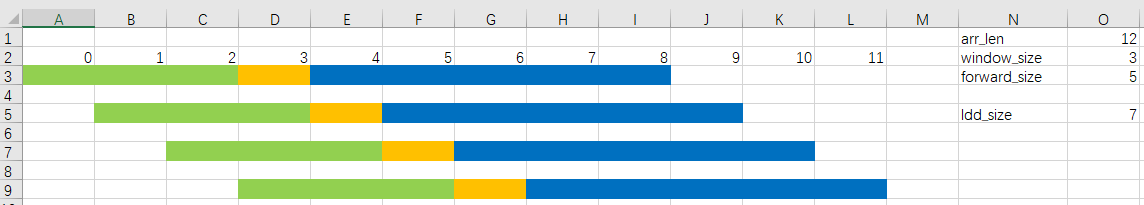
\includegraphics[width=10cm]{images/f000003}
    \end{figure}
    \item 第28$\sim$34行:起点为window\_size,如上图行3橙色单元格,终点为ldd\_size=length-forward\_size=12-5=7,不包括该值,每步循环时,当前时刻向右移一格,
    将前面window\_size=3个时间点数据加入到item中,最后将当前时间点pos加入到item中,最后将item作为一个样本,加入到原如数据集中;
    \item 第35$\sim$37行:将其转变为np.ndarray,并保存到如sh600260\_1m\_X.csv中;
    \item 第39、40行:生成与X同长度的y,每个时间点是一个0、1、2中三个数中的一个数,分别代表上涨、下跌和震荡,具体实现在下面的进行详细介绍;
    \begin{figure}[H]
        \caption{读取原始行情数据原理示意图}
        \label{f000004}
        \centering
        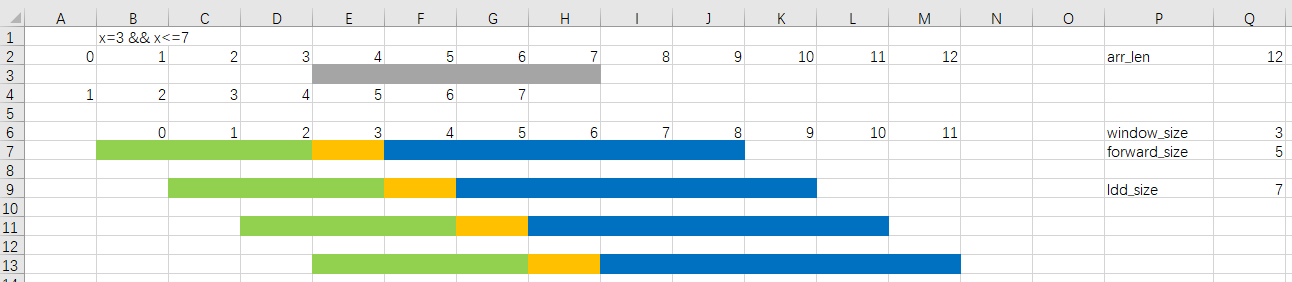
\includegraphics[width=10cm]{images/f000004}
    \end{figure}
    \item 第42$\sim$52行:由于我们在上步读取数据集时,针对的是一阶对数差分序列,所以其比原始数据(上图上部)少一列数据。
    \begin{itemize}
        \item 初始时seq=0,不满足if条件,不处理第0时刻数据,seq=1;
        \item seq=1不满足if条件,不处理第1时刻数据,seq=2;
        \item seq=2不满足if条件,不处理第2时刻数据,seq=3;
        \item seq=3不满足if条件,不处理第3时刻数据,seq=4;
        \item seq=4满足if条件,将第4时刻数据加入到行情数据中,seq=5;
        \item seq=5满足if条件,将第5时刻数据加入到行情数据中,seq=6;
        \item seq=6满足if条件,将第5时刻数据加入到行情数据中,seq=7;
        \item seq=7满足if条件,将第5时刻数据加入到行情数据中,seq=8;
        \item seq=8满足if条件,将第5时刻数据加入到行情数据中,seq=9;
        \item ......;
    \end{itemize}
    \item 第54行:返回X、y和原始行情数据raw\_datas;
\end{itemize}
\subsection{确定市场行情}
下面我们来看怎样根据前10个时刻及当前时刻的行情数据,确定在未来是上涨、下跌或震荡行情,从而根据仓位选择合理的操作。
\lstset{language=PYTHON, caption={确定当前时刻市场状态}, label={c001-determine-market-state}, basicstyle = \ttfamily}
\begin{lstlisting}
# apps/fmts/ds/ohlcv_processfor.py
    @staticmethod
    def get_market_state(y: np.ndarray, quotation: np.ndarray, window_size: int, forward_size: int) -> None:
        '''
        针对收盘价,从window_size处开始,向后看forward_size条记录,上限为当前收盘价*1.01,下限为当前收盘价*0.95,当
        在forward_size窗口内收盘价高于上限时返回0表示上升行情需要买入,低于下限时返回1表示下跌行情需要卖出,
        否则返回2表示震荡行情,将该值写入y中
        '''
        cnt = y.shape[0]
        q_cnt = quotation.shape[0]
        for idx in range(0, cnt, 1):
            curr_price = quotation[idx+window_size][3]
            high_limit = curr_price * 1.01
            low_limit = curr_price * 0.995
            market_regime = 2
            for pos in range(idx+window_size+1, idx+window_size+1+forward_size, 1):
                future_price = quotation[pos][3]
                if future_price >= high_limit:
                    market_regime = 0
                elif future_price <= low_limit:
                    market_regime = 1
            y[idx] = market_regime


# 测试程序:utcs/apps/fmts/ds/t_ohlcv_processor.py
    def test_get_market_state002(self):
        # 开始下标:window_size,结束下标:cnt-forward_size-1(包含)
        random.seed(1.0)
        y = np.zeros((10,), dtype=np.int64)
        quotation_raw = []
        cnt_y = 10
        curr_price = 5.36
        high_delta = 1.01
        low_delta = 0.995
        window_size = 3
        forward_size = 4
        cnt = cnt_y+window_size+forward_size
        for idx in range(cnt):
            close_price = random.uniform(curr_price*low_delta, curr_price*high_delta)
            item = [0.01, 0.02, 0.03, close_price, 0.04]
            quotation_raw.append(item)
        print('quotation_raw: {0}: {1};'.format(len(quotation_raw), quotation_raw))
        quotation = np.array(quotation_raw)
        OhlcvProcessor.get_market_state(y, quotation, window_size, forward_size)
        print('y: {0}; {1};'.format(y.shape, y))
        plt.ion()
        fig, axes = plt.subplots(1, 1, figsize=(8, 4))
        for idx in range(cnt_y):
            plt.draw()
            plt.pause(0.1)
            plt.cla()
            # 绘制价格变化曲线
            x = range(cnt)
            close_prices = [ix[3] for ix in quotation]
            plt.plot(x, close_prices, color='goldenrod', marker='*')
            # 绘制最左侧竖线
            low_limit = quotation[idx+window_size][3]*low_delta
            high_limit = quotation[idx+window_size][3]*high_delta
            x1 = np.array([idx+window_size, idx+window_size])
            y1 = np.array([low_limit, high_limit])
            plt.plot(x1, y1, color='darkblue', marker='o')
            # 绘制上限
            x2 = np.array([idx+window_size, idx+window_size+forward_size])
            y2 = np.array([high_limit, high_limit])
            plt.plot(x2, y2, color='darkblue', marker='o')
            # 绘制下限
            x3 = np.array([idx+window_size, idx+window_size+forward_size])
            y3 = np.array([low_limit, low_limit])
            plt.plot(x3, y3, color='darkblue', marker='o')
            # 绘制右侧竖线
            x4 = np.array([idx+window_size+forward_size, idx+window_size+forward_size])
            y4 = np.array([low_limit, high_limit])
            plt.plot(x4, y4, color='darkblue', marker='o')
            # 标注市场状态
            plt.title('市场状态:{0};'.format(y[idx]))
            msg = input('please input msg:')
        plt.show(block=True)
\end{lstlisting}
代码原理如下图所示:
\begin{figure}[H]
    \caption{确定市场行情状态代码原理示意图}
    \label{f000005}
    \centering
    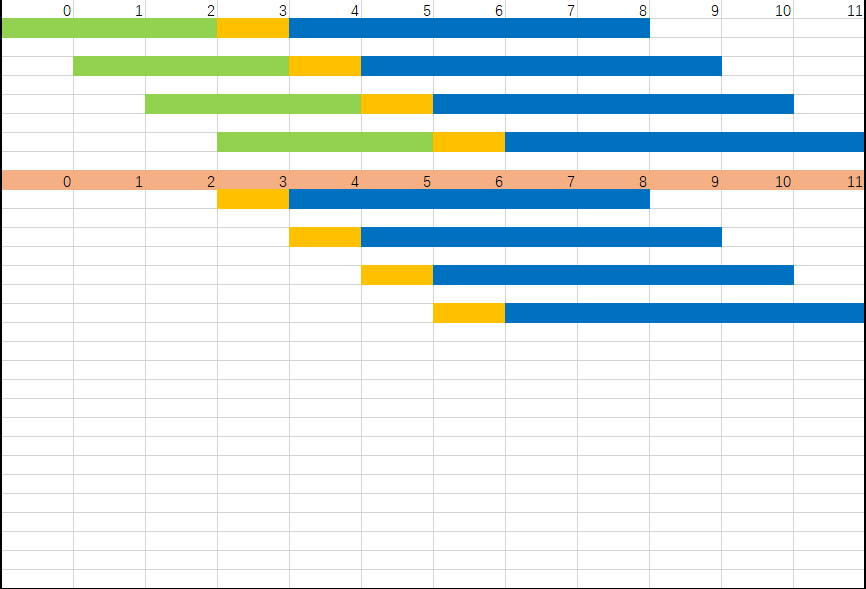
\includegraphics[width=10cm]{images/f000005}
\end{figure}
代码解读如下所示:
\begin{itemize}
    \item 第1行:;
    \item 第2行:;
    \item 第3行:;
\end{itemize}

\section{总结}